\chapter{预备知识}
Ren'Py是一种视觉小说语言,名字是恋愛(れんあい,即恋爱)与Python两词混合而成。Python是Ren'Py使用的编程语言。而 \textit{《心跳!心跳!文学部!》(Doki Doki Literature Club!},下文简称DDLC)正是基于Ren'Py编写的。想要编写DDLC Mod,我们就必须先学习Ren'Py相关知识。

本章将为您介绍Ren'Py的来源及如何安装Ren'Py与代码编辑器。

\section{关于Ren'Py}
\subsection{Ren'Py概述}
Ren'Py几乎支持视觉小说所应该具有的功能,如:分支故事、存储与加载游戏、回退到之前故事的存储点、多样性的场景转换等。其首次发布于2004年8月24日。Ren'Py拥有类似电影剧本的语法,并且能够允许用户编写Python代码来增加新的功能。除此之外,游戏引擎内附的出版工具能提供基本的脚本加密与压缩游戏素材。

Ren'Py建构于Python软件库Pygame之上,而它又基于了SDL。Ren'Py官方支持Windows、Linux以及较新版Mac OS X,并可通过Arch Linux、Ubuntu、Debian或Gentoo的软件包管理系统安装。它可以在Windows、macOS、Linux、Android、OpenBSD、iOS和wasm的HTML5下建置。

利用Ren'Py结合剧本及Python,我们可以制作出各种各样的游戏。Ren'Py也有一些电子角色扮演游戏框架的示例,但相对来说,制作RPG游戏会比较困难。

\section{下载Ren'Py}
目前主流的Ren'Py分为3个版本:Ren'Py 6、Ren'Py 7、Ren'Py 8。其中Ren'Py 6与Ren'Py 7兼容Python 2且Ren'Py 7已经支持大部分Python 3特性,而Ren'Py 8完全兼容Python 3。需要注意的是,Ren'Py 6已停止支持。

Ren'Py几乎可在所有主流系统上运行。由于Ren'Py 8目前稳定性存疑,故本书主要使用Ren'Py 7进行教学。

\begin{Comment}
Ren'Py 7.4.4及以后的版本均不支持Windows XP及更早的系统。
\end{Comment}

\subsection{下载Ren'Py SDK 7}\label{sec:1.2.1}
\begin{figure}[htbp]
    \centering
    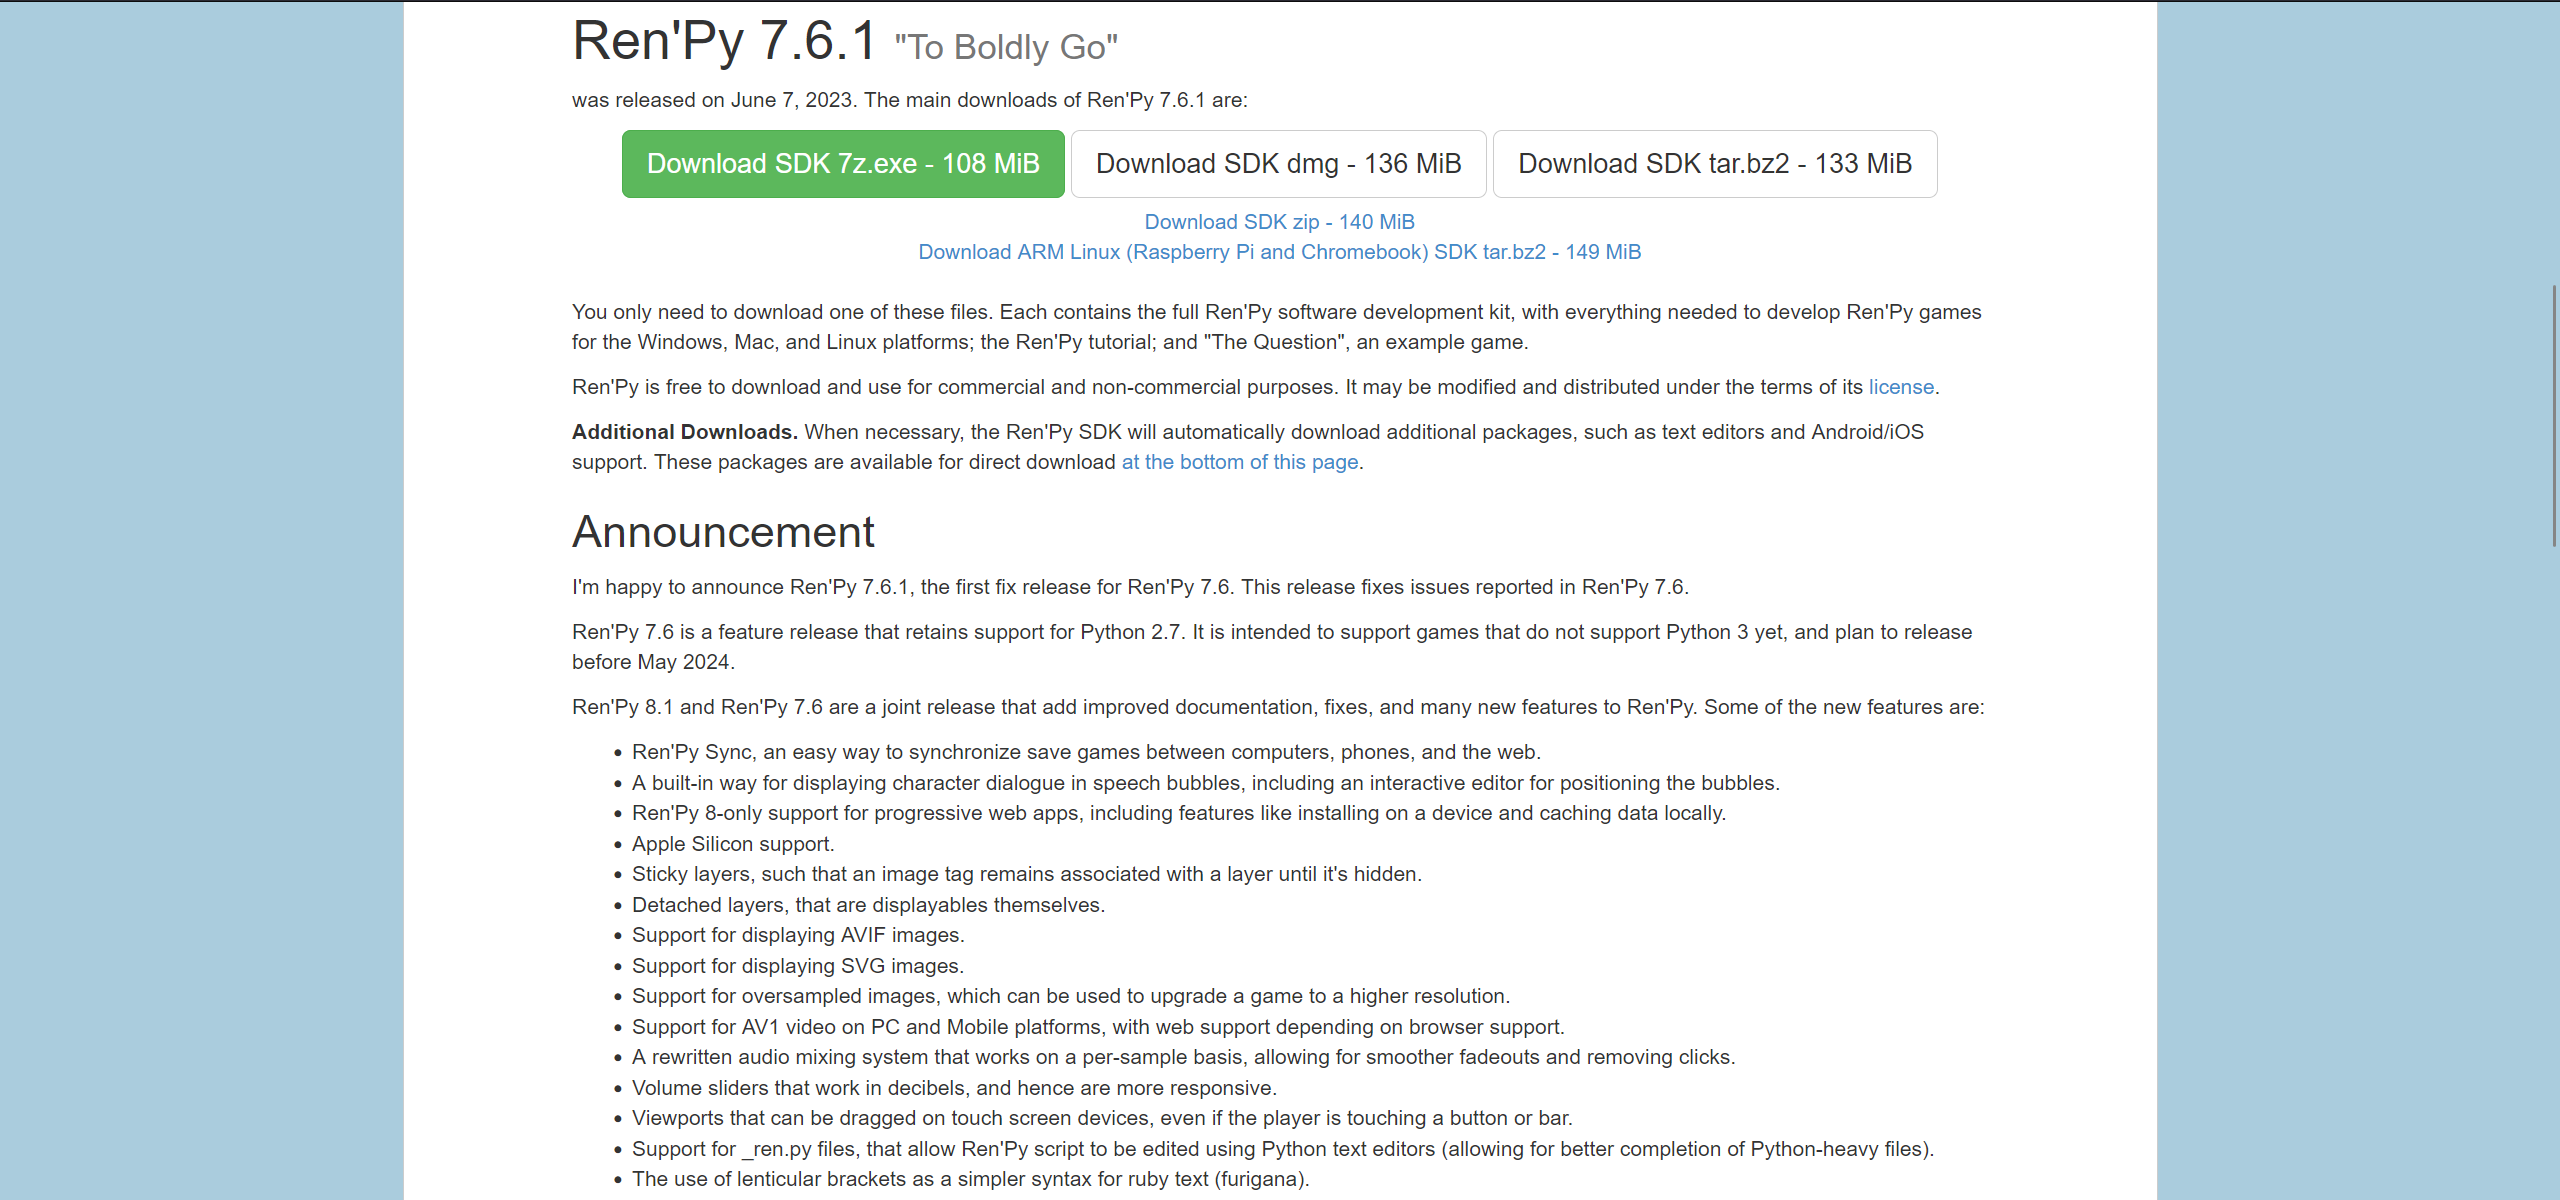
\includegraphics[scale=.3]{Pictures/1/1.2/1.2.1}
    \caption{Ren'Py官网}
    \label{fig:1.1}
\end{figure}

\begin{Comment}
本章编写时DDLC Mod中文模板支持的最新版Ren'Py SDK 7为7.6.1。
\end{Comment}
使用任意浏览器进入 \url{https://www.renpy.org/release/7.6.1} 网页(如图\ref{fig:1.1}),您将在本页面看到三个按钮,分别是:Download SDK 7z.exe、Download SDK dmg与 Download SDK tar.bz2。Windows用户请下载第一个,macOS用户请下载第二个,Linux用户请下载第三个。

\begin{Comment}
    若无法打开文件,请点击第二行小字Download SDK zip下载ZIP文件
\end{Comment}

\begin{figure}[htbp]
    \begin{minipage}{200pt}
        \centering
        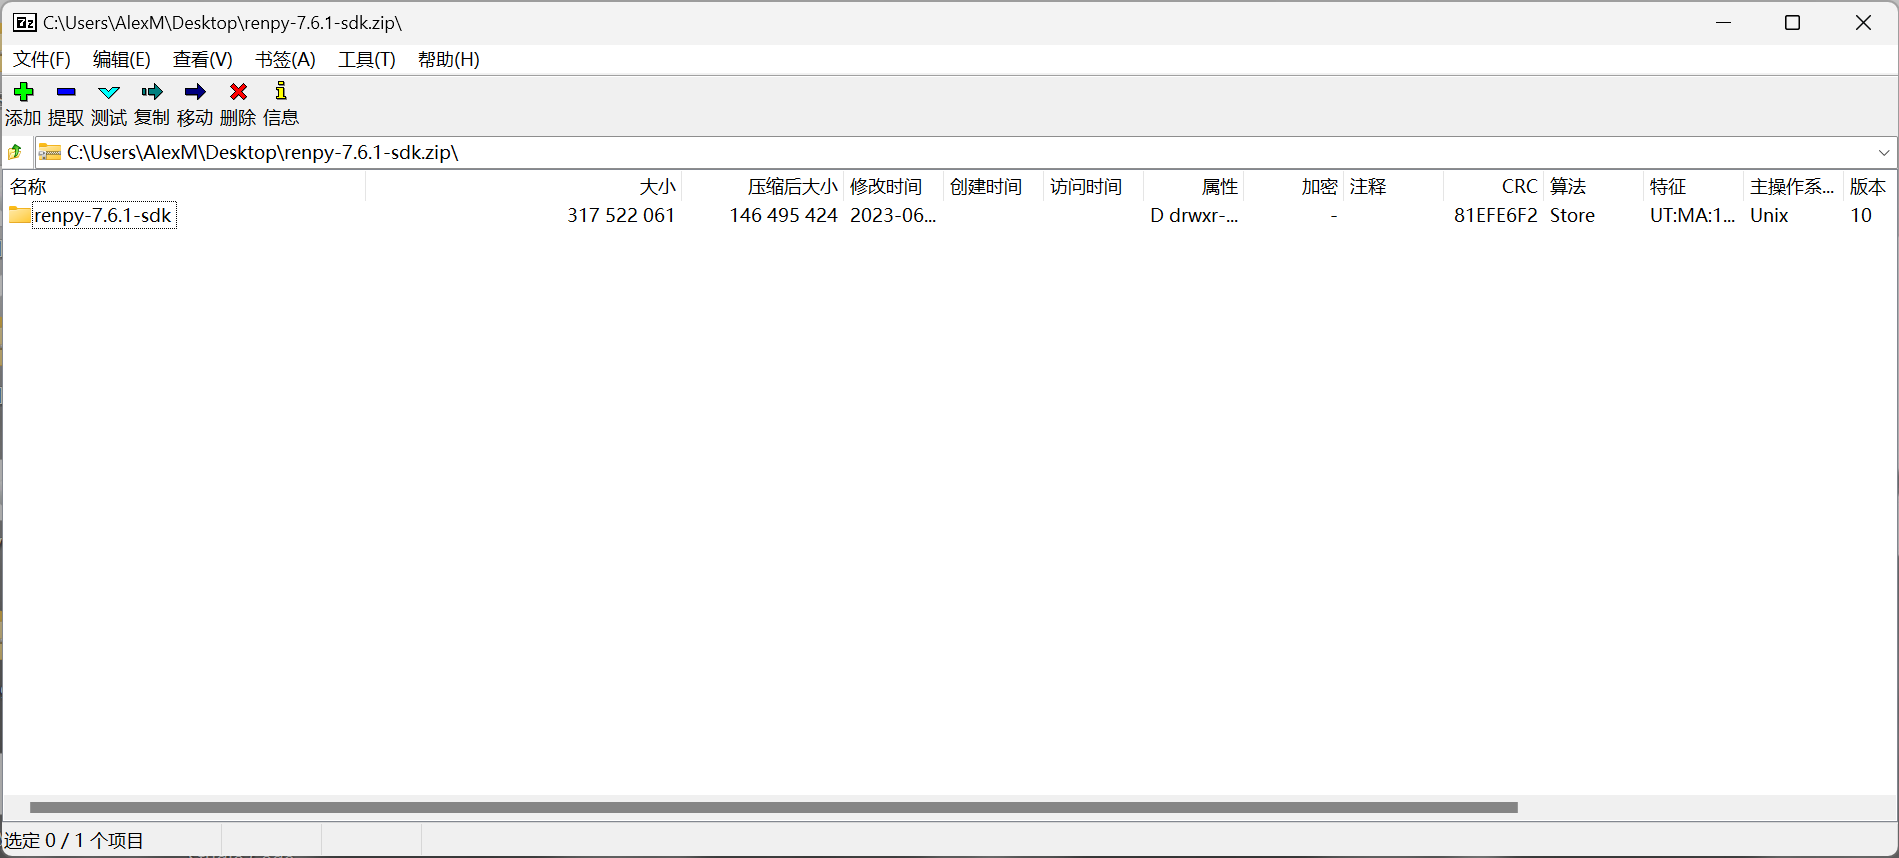
\includegraphics[scale=.2]{Pictures/1/1.2/1.2.2.png}
        \caption{ZIP文件}
        \label{fig:1.2}
    \end{minipage}
    \begin{minipage}{180pt}
        \centering
        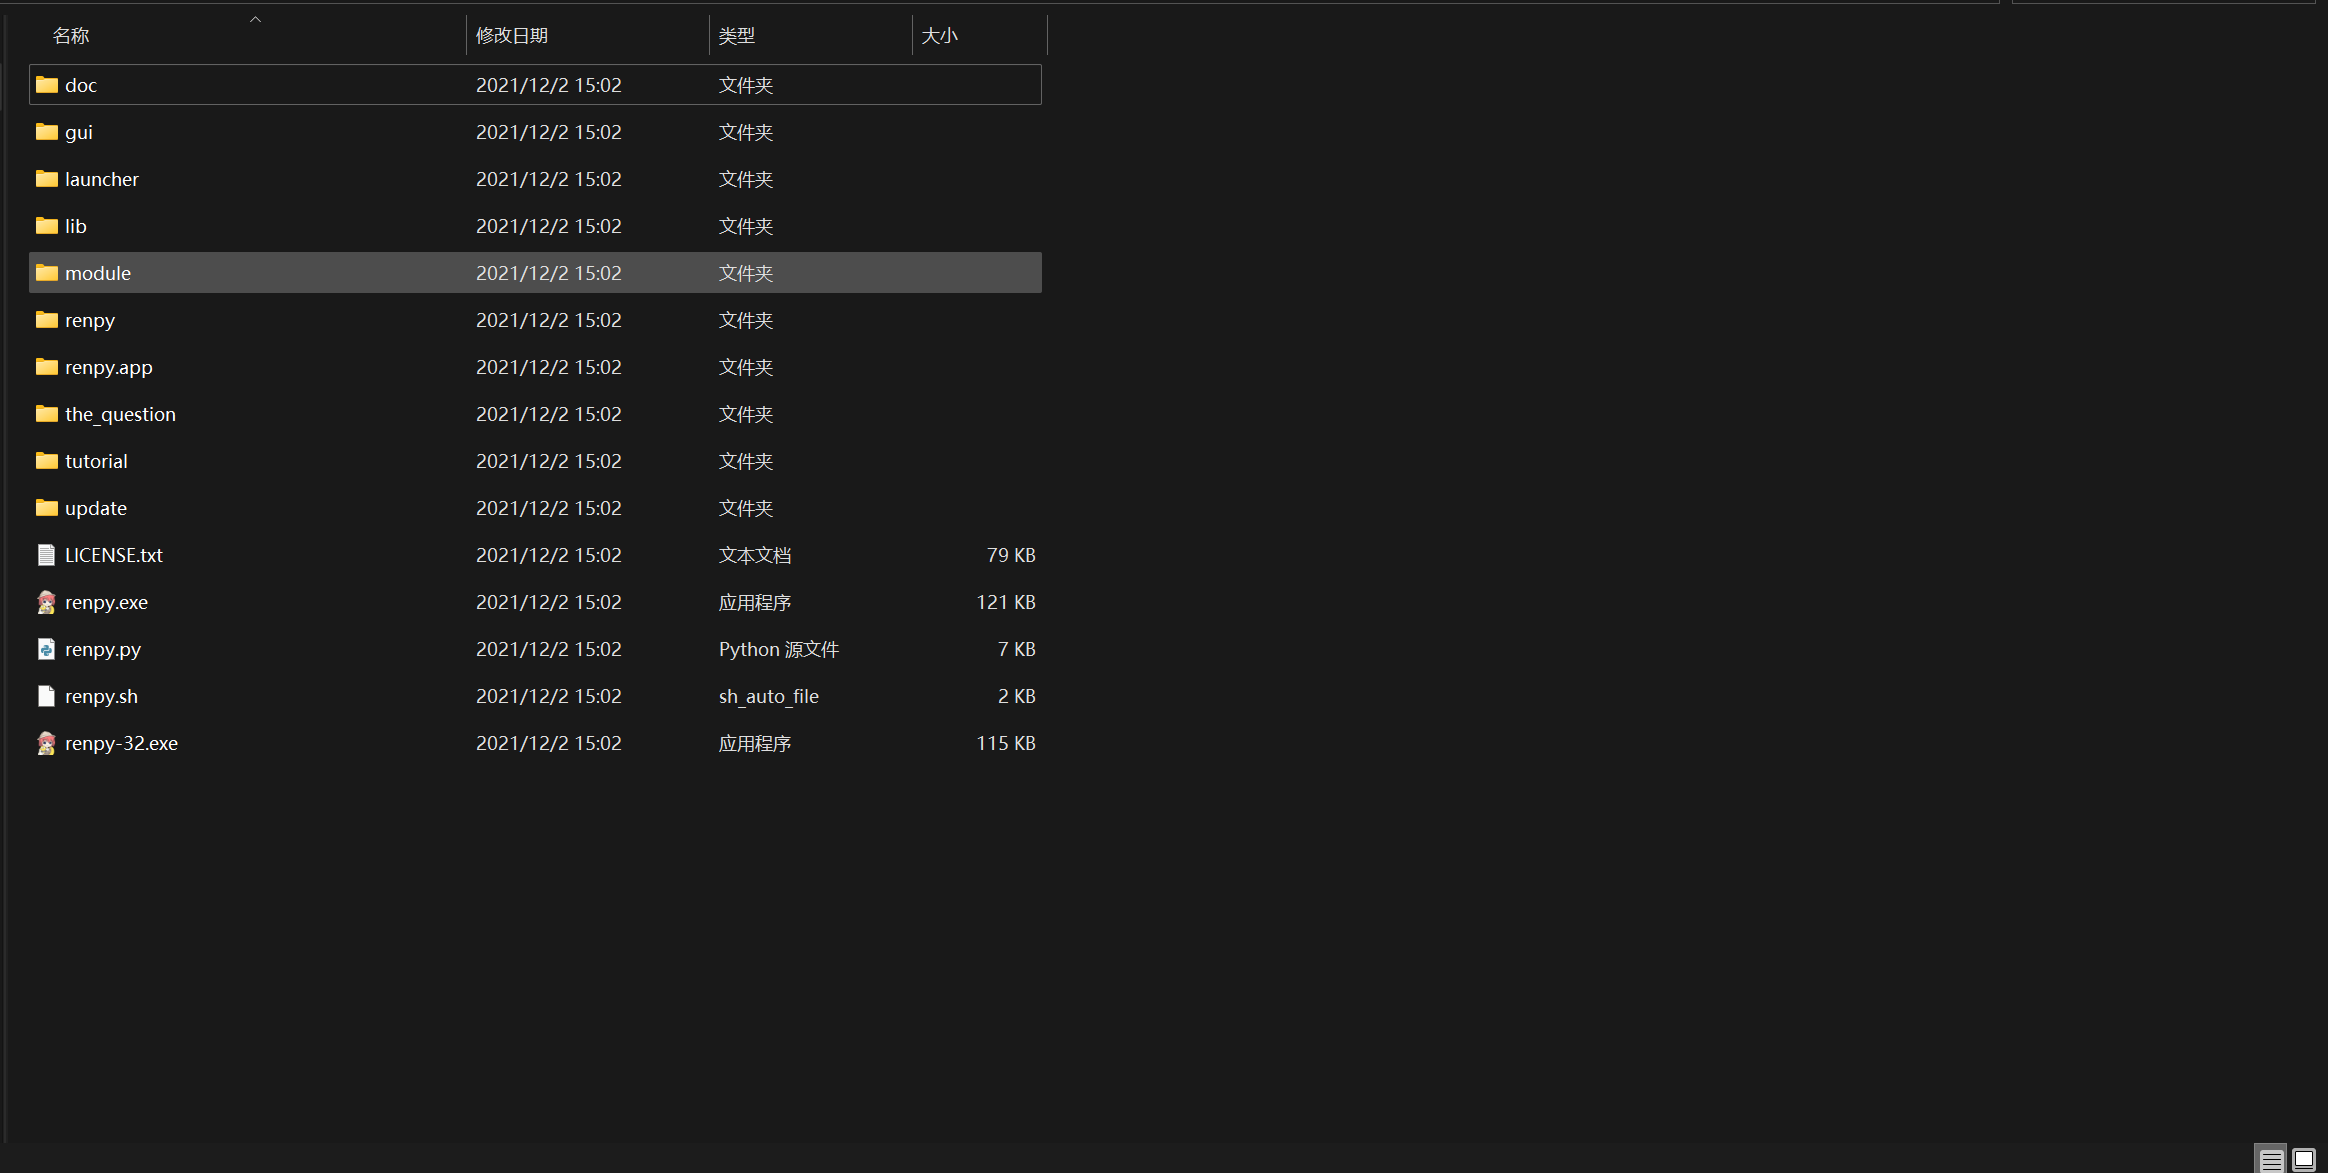
\includegraphics[scale=.15]{Pictures/1/1.2/1.2.3.png}
        \caption{文件夹内容}
        \label{fig:1.3}
    \end{minipage}
\end{figure}
以ZIP文件为例,下载完成后打开压缩包(如图\ref{fig:1.2})
将文件夹中的所有内容解压,得到如下内容。(如图\ref{fig:1.3})

Windows用户请双击renpy.exe或renpy-32.exe(在某些情况下,它可能显示为renpy或renpy-32);MacOS用户若使用驱动器镜像(dmg)安装Ren'Py,请运行renpy,否则运行 renpy.sh;Linux用户请运行renpy.sh。

\begin{figure}[htbp]
    \centering
    \begin{minipage}{182pt}
        \centering
        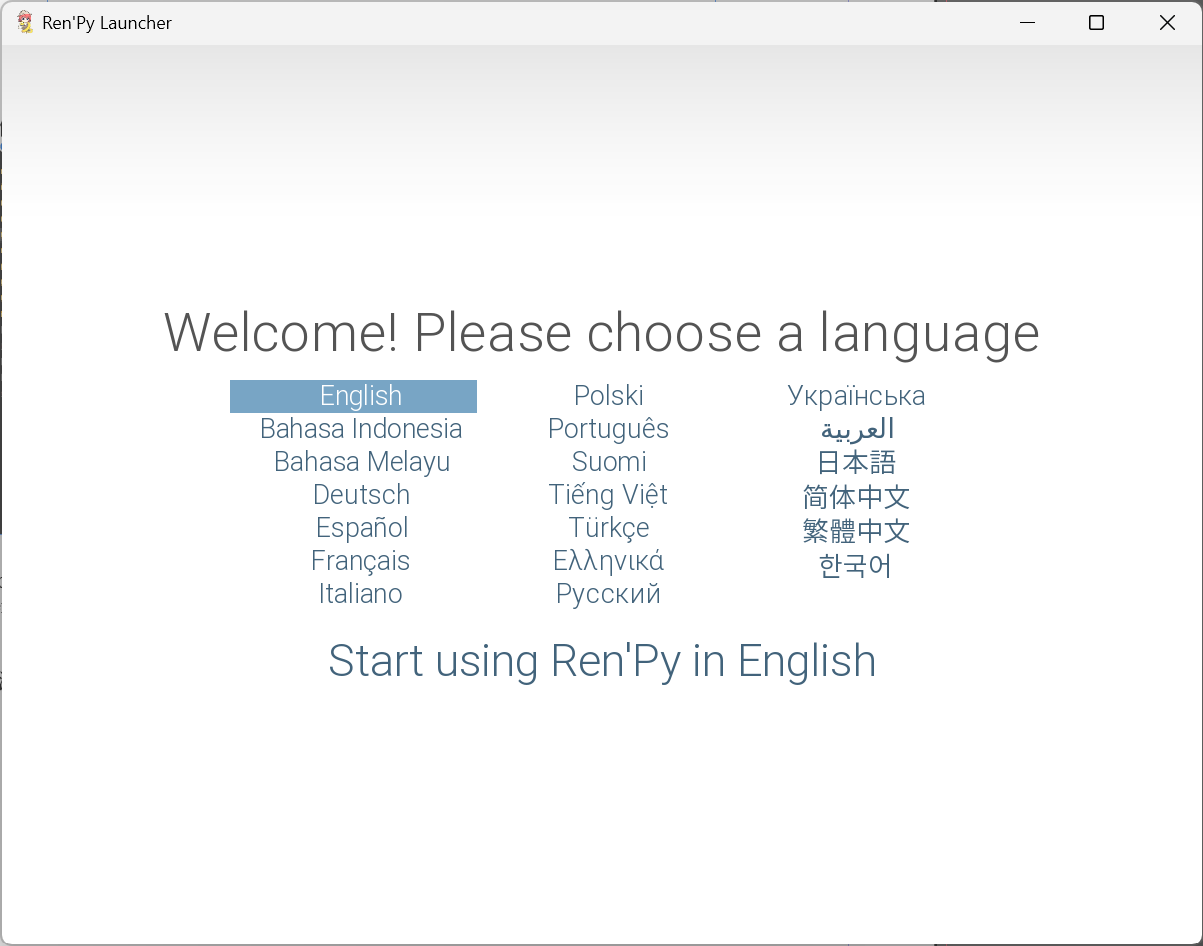
\includegraphics[scale=.2]{Pictures/1/1.2/1.2.4.png}
        \caption{选择语言}
        \label{fig:1.4}
    \end{minipage}
    \hspace{10pt}
    \begin{minipage}{182pt}
        \centering
        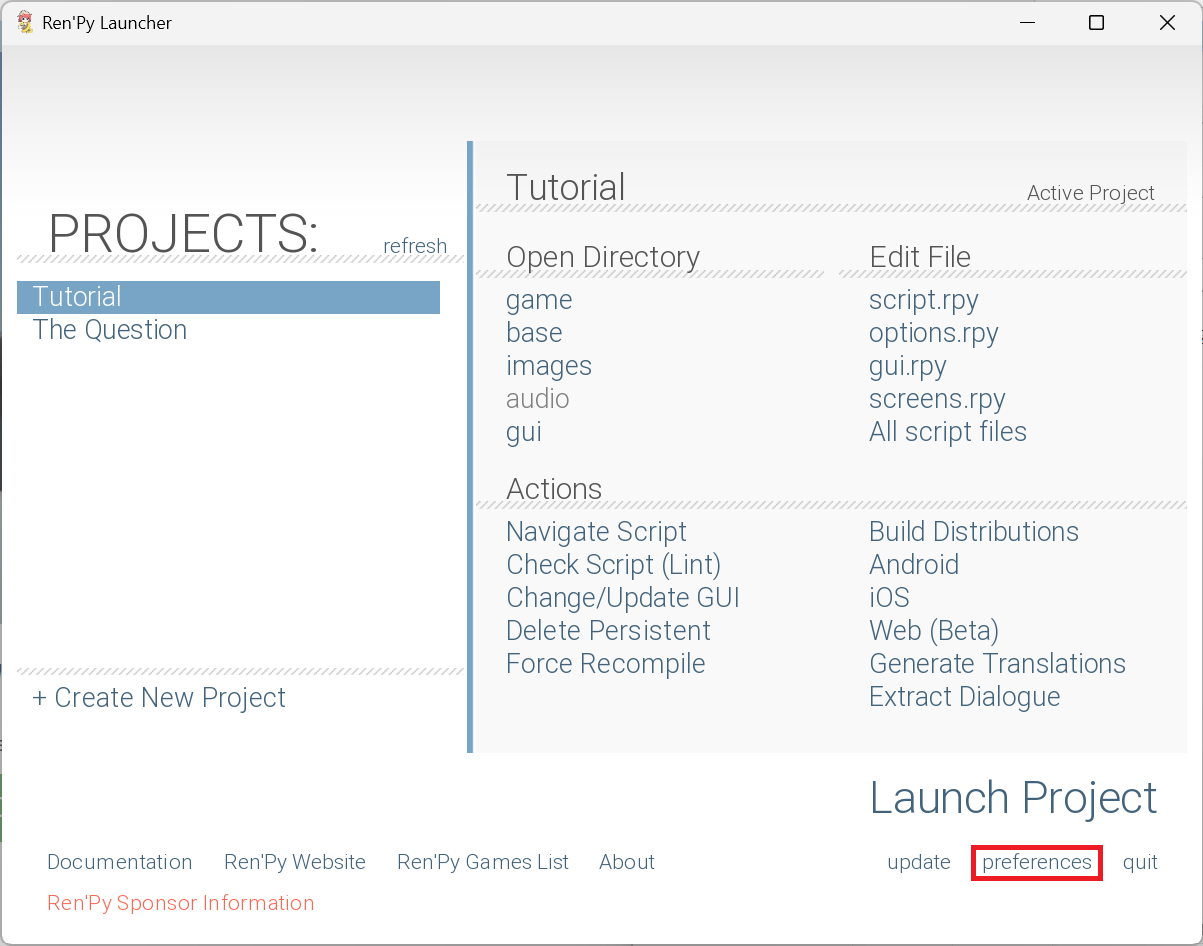
\includegraphics[scale=.2]{Pictures/1/1.2/1.2.5.png}
        \caption{调整语言}
        \label{fig:1.5}
    \end{minipage}
\end{figure}

打开Ren'Py后,正常来讲,您会见到如图\ref{fig:1.4}所示的界面。点击简体中文后,您会见到如图\ref{fig:1.5}所示的界面。

若您没有见到该界面,而是直接见到类似图\ref{fig:1.5},请点击右下角的preferences,在右下角Language中选中简体中文即可调整为简体中文。
